\section{Phương pháp đề xuất}\label{sec:method}
\subsection{Khung hệ thống}\label{sec:system}
Gọi $V$ là miền trạng thái hữu hạn của mạng đường có hướng, với tọa độ chiếu
$a_v$. Khoảng cách Euclid dùng cho privacy/định vị; chi phí có hướng dùng để
kiểm tra đường đi và xếp hạng dịch vụ. GPS $x_t$ và nhu cầu $\psi_t$ chỉ ở local.
Nhà cung cấp biết thuật toán và ngữ cảnh công khai $C$, đồng thời quan sát
tọa độ Q theo thứ tự, đồng hồ, truy vấn chung, phản hồi và lần thử lại.
Họ không thấy điểm tham chiếu $Z$, belief, sổ ngân sách hay kết quả đã xếp hạng
(Hình~\ref{fig:system}).

\begin{figure}[!ht]\centering
\resizebox{\columnwidth}{!}{\begin{tikzpicture}[>=Latex,
 box/.style={draw=ink!65,rounded corners=2pt,fill=white,text width=3.9cm,
 align=center,inner sep=5pt,font=\small},
 arr/.style={->,thick,draw=ink}]
\node[box,draw=teal,fill=teal!4] (model) at (0,0)
{\textbf{Thiết bị: GeoI-BQ}\\GPS riêng $\to Z$/belief $\to$ Q};
\node[box] (local) at (0,-1.7)
{\textbf{Xử lý đáp án tại local}\\Cache; lọc/sắp xếp bằng GPS và $\psi$};
\node[box,text width=2.5cm] (server) at (5.5,-.7)
{\textbf{LBS / bên quan sát}\\Thấy Q, đồng hồ,\\truy vấn và phản hồi};
\node[box,text width=3.9cm] (context) at (0,1.45)
{\textbf{Ngữ cảnh thiết kế công khai}\\Đường và toàn bộ tham chiếu thử nghiệm};
\node[box] (out) at (0,-3.1)
{\textbf{Đầu ra cho người dùng}\\Toàn danh sách phù hợp đã sắp xếp};
\draw[arr] (context)--(model);
\draw[arr] (model.east)--node[above,font=\scriptsize,align=center]{truy vấn\\chung}(server.north west);
\draw[arr,blue] (server.south west)--node[below,font=\scriptsize]{POI}(local.east);
\draw[arr] (local)--(out);
\draw[arr,teal] (model.west)--++(-.4,0)|-(local.west);
\begin{scope}[on background layer]
\node[fit=(model)(local)(context)(out),draw=teal,fill=teal!2,rounded corners,inner sep=8pt] {};
\end{scope}
\end{tikzpicture}
}
\caption{Ranh giới giữa thiết bị tin cậy và nhà cung cấp. Prototype đã nạp toàn
bộ dữ liệu tham chiếu tĩnh mà nhà cung cấp thử nghiệm sử dụng.}\label{fig:system}
\end{figure}

Bảo đảm đòi hỏi miền hỗ trợ ứng viên chung và trọng số nền công khai dương
tại mỗi tiền tố hành động mở rộng, kể cả trạng thái làn của điểm giả; kernel
không gian lý tưởng; bit ngẫu nhiên Q mới, đều và độc lập; trạng thái phiên
đã cam kết, không thể quay lui và khôi phục đầy đủ các thành phần trước Q;
ranh giới phiên/đồng hồ công khai; cùng quy luật phản hồi có điều kiện của
nhà cung cấp khi truy vấn/lịch sử giống nhau. Di chuyển được coi là ngoại sinh.
Tài khoản/IP, thời điểm bắt đầu/kết thúc riêng tư và phản hồi tác động tới
di chuyển là các kênh cần xét thêm. Kết quả cache đòi hỏi metadata hợp lệ và
thứ tự xếp hạng chung. Số học nguyên ở bước Q tự nó chưa chứng nhận toàn bộ
triển khai có số thực dấu phẩy động~\cite{mironov}.

Bộ khởi tạo prototype có đầy đủ dữ liệu tham chiếu/phản hồi khớp nhà cung cấp
tĩnh. Mặt nạ POI đã nhận giới hạn câu trả lời được đo, nhưng chưa tạo cách ly
thông tin: client offline có cùng dữ liệu có thể trả lời chính xác mọi yêu
cầu tĩnh đã định nghĩa. Chi phí thu thập và cập nhật dữ liệu là vấn đề riêng.

\subsection{Luồng xử lý}
\subsubsection{Điểm tham chiếu và belief đã bảo vệ.}
Cơ chế hàm mũ trên đường (REM) lấy mẫu trực tiếp một trạng thái đường:
\begin{equation}
R_u(v\mid x)=
\frac{e^{-u\|x-a_v\|/2}}{\sum_{w\in V}e^{-u\|x-a_w\|/2}},
\quad Z=a_v. \label{eq:rem}
\end{equation}
Ở lần đọc GPS tiếp theo được phép, tham chiếu cũ $h$ được kiểm tra bằng
\begin{equation}
D_t=\mathbf1\{\|x_t-h\|+\xi_t>\theta\},
\quad \xi_t\sim\operatorname{Lap}(0,1/u). \label{eq:test}
\end{equation}
Tái sử dụng tốn $u$; kiểm tra rồi tạo mới tốn $2u$; REM ban đầu tốn $u$.
Bộ lọc ngân sách dự phòng chi phí tối đa của bước kế tiếp trước khi đọc GPS:
\begin{equation}
u\sum_i c_i\le Mu\le C_s,\qquad
M=\lfloor C_s/u\rfloor,\quad c_i\in\{0,1,2\}. \label{eq:cap}
\end{equation}
Cấu hình đã đóng băng dùng $u=B/(2H_{\rm cfg})$,
$B=0.24\,\mathrm m^{-1}$ và $H_{\rm cfg}=12$, suy ra $u=0.01\,\mathrm m^{-1}$,
$M=23$, $C_s=0.23\,\mathrm m^{-1}$ và $\theta=200$ m.
Tổng quát, $C_s\le\log(R_\star)/d_\star$ đủ để chặn tỷ số không gian bởi
$R_\star$ khi $D_\infty\le d_\star$. Hết ngân sách sẽ ngừng đọc GPS cho cơ chế
bảo vệ, nhưng không ngừng gửi truy vấn.

Belief trên các trạng thái đại diện dự đoán bằng mô hình di chuyển công khai
và chỉ cập nhật khi thực sự có quan sát đã bảo vệ:
\begin{align}
b_t^-(s)&=\sum_r b_{t-1}(r)T_{\Delta t}(r,s),\\
b_t(s)&\propto b_t^-(s)\ell_t(Z_t\mid s,h). \label{eq:belief}
\end{align}
Hàm phát xạ kết hợp khối xác suất tại tham chiếu được tái sử dụng với xác suất
REM khi tạo mới. Bỏ qua lần đọc thì chỉ dự đoán; Z lặp lại không phải phép
đo độc lập. Belief xấp xỉ này chưa được chứng nhận hiệu chuẩn trên người dùng thật.

\subsubsection{Chọn đoạn truy vấn và trả lời local.}
Mỗi hành động gồm ba khung K5 (mỗi khung năm điểm Q), nối nhau bằng chuyển
động khả thi trên đường có hướng. Ngữ cảnh công khai cùng hành động/phản hồi
giả trước đó xác định thư viện và trọng số; GPS, Z, belief và request không
được dùng để loại ứng viên khỏi miền hỗ trợ. Đứng yên cung cấp lựa chọn khả
thi chung; nếu xây dựng thư viện công khai rỗng thì ghi nhận là thất bại.
Bộ lập kế hoạch đã đóng băng dùng độ rộng 24, trọng số mới lạ/tầm xa bằng bốn
và thang di chuyển 60 s. Tài liệu bổ sung đặc tả trọng số cùng điểm đại diện
$g_a(s)$ bị chặn, dựa trên độ phủ cache và độ gần.

Điểm $v_a=\sum_sb(s)g_a(s)$ được chuẩn hóa/lượng tử thành $z_a\in[0,1]$
với độ phân giải 65536. Tại đoạn $j$,
\begin{align}
\varepsilon_{Q,j}&=\frac{\Gamma_Q}{j(j+1)},&
\alpha_j&=\frac{\widehat\varepsilon_{Q,j}}{2+\widehat\varepsilon_{Q,j}},\\
\mu_j&=\sum_aw_az_a,&
p_a&=w_a[1+\alpha_j(z_a-\mu_j)]. \label{eq:kernel}
\end{align}
Ở đây $\widehat\varepsilon_{Q,j}\le\varepsilon_{Q,j}$ là hạn mức hữu tỷ làm
tròn xuống; thực nghiệm dùng $\Gamma_Q=1$. Trọng số tích lũy nguyên chính xác
thực hiện phân phối này với điều kiện các bit đầu vào đều.

Đoạn đã cam kết phát các khung tại 0, 20 và 40 s; đoạn tiếp theo bắt đầu ở
60 s (Hình~\ref{fig:model}). Các lần đọc GPS cho cơ chế bảo vệ cách nhau ít
nhất 60 s; GPS local hiện tại vẫn có thể dùng xếp hạng ở mỗi nhịp dịch vụ.
Mỗi Q yêu cầu cùng sáu loại POI, $L60$ cho mỗi loại. Thiết bị loại trùng/lưu
cache, sau đó lọc và sắp xếp riêng theo $\psi_t$. Người dùng nhận toàn bộ danh
sách phù hợp; top năm chỉ là tập tham chiếu khi đánh giá.

\begin{figure*}[t]\centering
\resizebox{.94\textwidth}{!}{\begin{tikzpicture}[>=Latex,
 box/.style={draw=ink!65,rounded corners=2pt,fill=white,text width=4cm,
 align=center,inner sep=6pt,font=\small},
 side/.style={draw=blue!60,fill=blue!4,rounded corners=2pt,text width=4cm,
 align=center,inner sep=5pt,font=\small},
 arr/.style={->,thick,draw=ink}]
\node[box] (rem) at (0,0)
{\textbf{1. Lịch sử không gian đã bảo vệ}\\Đọc GPS khi được phép: REM $Z$\\Kiểm tra giữ/đổi riêng tư; giới hạn $C_s$};
\node[box] (belief) at (5.6,0)
{\textbf{2. Belief từ dữ liệu đã bảo vệ}\\Dự đoán chuyển động +\\cập nhật theo quan sát đã bảo vệ};
\node[box,draw=teal] (choose) at (11.2,0)
{\textbf{3. Chọn chung cả đoạn Q}\\Thư viện/nền chung; hiệu chỉnh có cận\\Lưu bền bộ đếm $j$ và hành động};
\node[box] (send) at (11.2,-2.1)
{\textbf{4. Cam kết và công bố}\\K5 tại 0/20/40 s; đoạn mới tại 60 s\\Truy vấn sáu loại chung, L60};
\node[box] (local) at (5.6,-2.1)
{\textbf{5. Xử lý dịch vụ tại local}\\Hợp/cache các POI hợp lệ\\Lọc/sắp xếp bằng GPS hiện tại + $\psi$};
\node[side] (input) at (0,1.7)
{\textbf{Luồng GPS riêng tư}};
\node[side,text width=6.9cm] (public) at (8.4,1.7)
{\textbf{Ngữ cảnh công khai:} đường, proxy, đồng hồ, Q/phản hồi trước};
\node[side] (output) at (0,-2.1)
{\textbf{Đầu ra}\\Toàn danh sách phù hợp đã sắp xếp};
\node[side] (provider) at (11.2,-3.8)
{\textbf{LBS bên ngoài:} Q $\to$ POI};
\draw[arr] (input)--(rem);
\draw[arr] (rem)--(belief);
\draw[arr] (belief)--(choose);
\draw[arr] (choose)--(send);
\draw[arr] (local)--(output);
\draw[arr,blue] (send)--(provider);
\draw[arr,blue] (provider.west)-|node[below,pos=.3,font=\scriptsize]{phản hồi POI}(local.south);
\draw[arr,dashed,blue] (public.south west)--(belief.north);
\draw[arr,dashed,blue] (public.south east)--(choose.north);
\draw[arr,dashed] (local.north)--(5.6,-1.05)-|(choose.west);
\node[font=\scriptsize,fill=white,inner sep=2pt] at (7.3,-1.05) {chỉ cache công khai};
\begin{scope}[on background layer]
\node[fit=(rem)(belief)(choose)(send)(local),draw=teal,fill=teal!2,
 rounded corners,inner sep=10pt] (boundary) {};
\end{scope}
\node[font=\scriptsize\bfseries,text=teal,anchor=north west,fill=white,inner sep=2pt]
at (boundary.north west) {GEOI-BQ TRÊN THIẾT BỊ};
\end{tikzpicture}
}
\caption{Luồng GeoI-BQ. Lịch sử không gian đã bảo vệ chấm điểm cho thư viện
đoạn công khai chung; các khung đã cam kết truy hồi POI để xếp hạng local.
Chỉ thông tin cache công khai được dùng lại khi tạo ứng viên.}\label{fig:model}
\end{figure*}

Hình~\ref{fig:walkthrough} theo dõi một chuyến TEST đã lưu, được chọn vì
đường đi có nhiều lần rẽ. Tại 20/40 s, belief chỉ dự đoán, không đọc GPS cho
cơ chế bảo vệ; kiểm tra rồi tạo mới tại 60/120/180 s đều tốn hai đơn vị.

\begin{figure*}[t]\centering
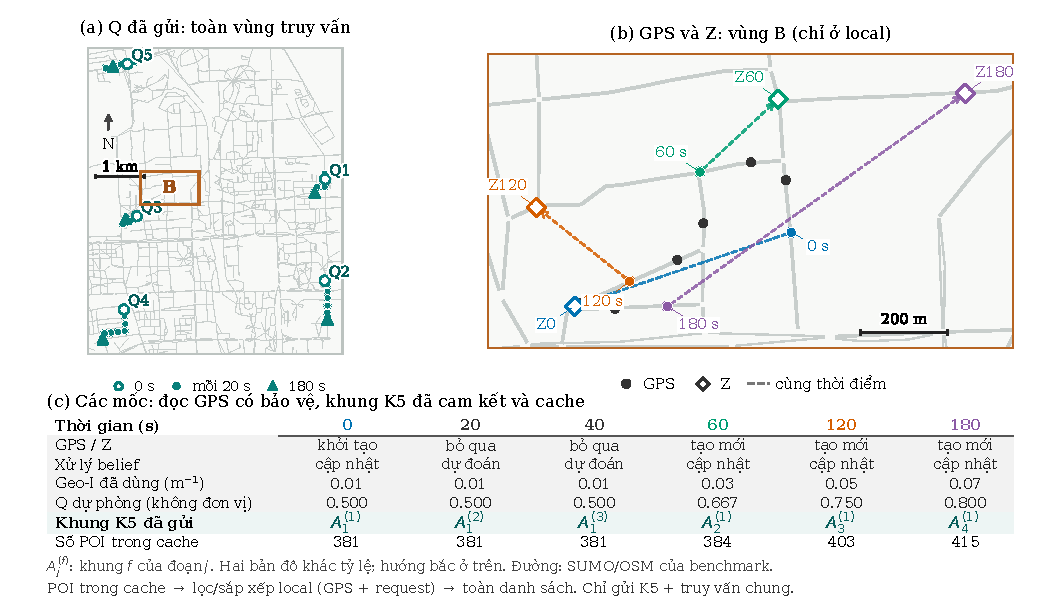
\includegraphics[width=\textwidth]{figure_walkthrough.pdf}
\caption{Chuyến đã lưu \texttt{cache-046\_day7}, 0--180 s.
(a) Cả năm luồng Q; khung B định vị phần phóng lớn riêng ở (b).
GPS tô đặc và Z rỗng có nhãn/màu theo cùng thời điểm; nét đứt thể hiện độ
lệch tham chiếu, không phải đường di chuyển.
(c) Một số mốc và khung đã cam kết; ba khung đầu thuộc cùng đoạn.
Z, belief, sổ ngân sách và kết quả đã xếp hạng đều ở local.}\label{fig:walkthrough}
\end{figure*}
